\chapter{System architecture}
CERMINE workflowed is composed of a multi-part pipeline, out of which every stage is treated as a separate module and can be maintained and developped independently. For implementation of the majority of non-trivial problems we used supervised and unsupervised machine learning algorithms, that gave a lot of elasticity and allow to adapt to new document layouts.

\quad
CERMINE workflow consists of the following distinguishable stages:
\begin{enumerate}
    \item \textbf{Text extraction} takes place at the very beginning of metadata extraction process. CERMINE using pdfbox, an external library for manipulating PDF content, extracts a stream of characters, together with their geometrical properties, from the input files.
    \item \textbf{Text segmentation} builds up blocks of text from a set of characters using their position and size. This stage uses Docstrum algorithm, coded by Krzysztof Rusek and described in details in \cite{O'Gorman1993}. It is therefore beyond the scope of this work and will not be mentioned hereafter.
    \item \textbf{Resolution of the reading order} aims figuring out the order in which blocks of text are meant to be read. While this task is trivial to a human reader, it is tricky to implement an elastic algorithm suitable for different article layouts.
    \item \textbf{Basic structure extraction} takes a PDF file on the input and produces a geometric hierarchical structure representing the document. The structure is composed of pages, zones, lines, words and characters. The reading order of all elements is determined. Every zone is labelled with one of four general categories: \verb+METADATA+, \verb+REFERENCES+, \verb+BODY+ and \verb+OTHER+.
    \item \textbf{Metadata extraction} part analyses parts of the geometric hierarchical structure labelled as \verb+METADATA+ and extracts a rich set of document's metadata from it.
    \item \textbf{References extraction} part analyses parts of the geometric hierarchical structure labelled as \verb+REFERENCES+ and the result is a list of document's parsed bibliographic references.
    \item \textbf{Text extraction} part analyses parts of the geometric hierarchical structure labelled as \verb+BODY+ and extracts document's body structure composed of sections, subsections and paragraphs. 
\end{enumerate}
A diagram of the above mentioned workflow can be found in the figure \ref{fig:pipeline}.
\begin{figure}[h]
  \centering
  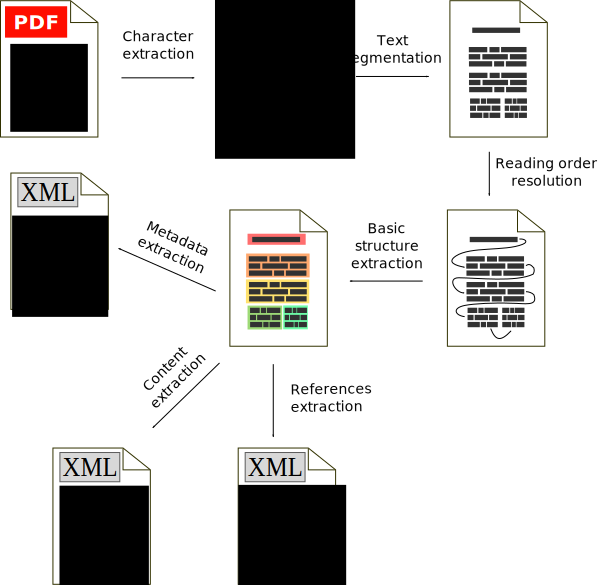
\includegraphics[width=14cm]{graphics/pipeline}
  \caption{A schematic diagram of CERMINE's workflow.}
  \label{fig:pipeline}
\end{figure}

\section{Structure extraction}
\subsection{Character extraction}\label{sec:character_extraction}
PDF document as such consists of a stream of characters, whereas position of each character in the stream doesn't have to be related, and usually is not, to its position in the text. Extraction of the characters is achieved using iText library. This part of the system was entirely implemented by Dominika Tkaczyk and will not be described in this work.
\subsection{Page segmentation}\label{sec:page_segmentation}
Page segmentation is a task of clustering a set of characters into blocks of text. Implemented system uses internally the Docstrum algorithm, described in details in \cite{O'Gorman1993}. It is a bottom-up approach based on
nearest-neighborhood clustering of connected components extracted from the document. $K$-neareast neigbours for each component are found and text lines are found based on a threshold of the angle between component centroids. Then, histograms of components spacing are used to detect inter-character distance in a word and between words. The algorithm has a set of thresholds that have to be set based on experiments with various documents. The algorithm was implemented by Krzysztof Rusek and tuned by Dominika Tkaczyk and therefore will not be described in this document in details.

\subsection{Reading order resolving}\label{sec:reading_order}
Resolution of Reading Order is a process aiming to transform text zones from a two-dimensional space (as they are laid out on the paper) to a single-dimensional space, i.e. as they are read by a human. Usually this is done by going from left to right and from top to bottom, but there are a lot of cases that made this na\"\i ve approach less efficient. This includes multi-column layout, page numbers, textual elements of figures, figures' and equations' labels.
\qquad
As already described in \cite{DominikaTkaczykPaweSzostekMateuszFedoryszakPiotrJanDendek2014}, a PDF file contains a stream of characters that undergoes processes of extraction and segmentation. This results in a list of pages consisting of zones, lines, words and chunks of text. These elements need to be put together in the same order as that would be done by a human reader.\\
To this end, a bottom-up strategy is applied: firstly characters are sorted within words and words within lines in ascending order according to X coordinate value. Afterwards, lines are sorted with Y coordinate as the key. As next we need to figure out zones' order. Below we describe a heuristic responsible for setting order of text zones Its fundamental principle was taken from \cite{ROR_source}. A schematic diagram of this phase can be found in the figure \ref{fig:reading_order}.
\begin{figure}[]
  \centering
  \includesvg[width=12cm]{graphics/ro}
  \caption{A schematic diagram of reading order resolving. Firstly, distances between text zones are calculated. Then, zones are hierarchicaly grouped according to distances between them. Finally, the tree is in-order traversed and a list of zones in created.}
  \label{fig:reading_order}
\end{figure}
\begin{enumerate}
\item For each pair of items inside a single page boundaries a free space between them is calculated. On the figure \ref{fig:reading_order} this space is ilustrated as the black area between two zones. The full implementation of the algorithm is included in the appendix \ref{appendix:ror}. Below is a detailed description of the steps taken.
	\begin{enumerate} 
	\item Formally the free space $S$ can be expressed as $S = A_d - (A_1+A_2)$, where $A_1$ and $A_2$ are areas of the two zones and $A_d$ is area of the smallest rectangle in which two objects can fit. This rectangle has to have sides parallel to the X and Y axes.
	\item To include preference for vertical clustering (and to avoid joining blocks horizontally when multi-column layouts are present) a cosine of the angle $\alpha$ between the vector $\vec{v}$ connecting two objects' geometrical centers and vector $\vec{x}$ being a projection of the vector $\vec{v}$ on the X axis is calculated. This was illustrated in the figure \ref{fig:angle_alpha}. The formula $\cos\alpha = \frac{\vec{v} \cdot \vec{x}}{|\vec{v}||\vec{x}|}$ is employed.
	\item Free space $S$ is multiplied by sum of coefficient $M$ and $\cos\alpha$. Coefficient $M$ is introduced in order to prevent situations when more than two zones have the same width and lay in-line with respect to the Y axes. Then, for each of them the calculated distance would be equal to zero. In such cases we prefer to join these two groups between which the Euclidean distance is minimized.
	\end{enumerate}
\item A list $L$ containing triples ($O_1$, $O_2$, $D$) is created (where $O_1$ and $O_2$ are zones on the page and $D$ is the distance between zones) Initially there are $\binom{N}{2}$ elements in the list.
\item List $L$ is sorted in ascending order with respect to the distance $D$. 
\item Until this list is empty, the first triple is picked (i.e. with the smallest distance $D$) and two associated objects, $O_1$ and $O_2$, are merged.
\item For each element $E$ in the $L$ recalculate the distance $D$ to the new group iff the $E$ contains $O_1$ or $O_2$ (i.e. is in form of ($O_1$, $X$, $D$) or ($O_2$, $X$, $D$)).  Insert into the list a new triple ($O_1O_2$, $X$, $D$) where $O_1O_2$ is the new group.
\item Sort the list $L$ in ascending order.
\end{enumerate}
\begin{figure}[h!]
  \centering
  \includesvg[width=8cm]{graphics/angle_alpha}
  \caption{To include preference for vertical clustering a cosine of the angle $\alpha$ between the vector $\vec{v}$ and vector $\vec{x}$ is calculated.}
  \label{fig:angle_alpha}
\end{figure}
\begin{lstlisting}[caption=Listing of the function measuring distance between two zones or zone groups.]

private double distance(BxObject obj1, BxObject obj2) {

    double x0 = Math.min(obj1.getX(), obj2.getX());
    double y0 = Math.min(obj1.getY(), obj2.getY());
    double x1 = Math.max(obj1.getX() + obj1.getWidth(),
            obj2.getX() + obj2.getWidth());
    double y1 = Math.max(obj1.getY() + obj1.getHeight(),
            obj2.getY() + obj2.getHeight());
    double dist = ((x1 - x0) * (y1 - y0) - obj1.getArea() - obj2.getArea());

    double obj1CenterX = obj1.getX();
    double obj1CenterY = obj1.getY() + obj1.getHeight() / 2;
    double obj2CenterX = obj2.getX();
    double obj2CenterY = obj2.getY() + obj2.getHeight() / 2;

    double obj1obj2VectorCosineAbs = Math.abs((obj2CenterX - obj1CenterX) / Math.sqrt((obj2CenterX - obj1CenterX) * (obj2CenterX - obj1CenterX) + (obj2CenterY - obj1CenterY) * (obj2CenterY - obj1CenterY)));
    final double M_COEFF = 0.5;
    return dist * (M_COEFF + obj1obj2VectorCosineAbs);
}
\end{lstlisting}
\section{Initial zone classification}
After the stages described in sections \ref{sec:character_extraction}, \ref{sec:page_segmentation} and \ref{sec:reading_order} the document can undergo the two phases of classification. Firstly, all the zones are classified to one of the four general classes: \verb+METADATA+, \verb+REFERENCES+, \verb+BODY+ and \verb+OTHER+. After this stage, more specific classifiers and algorithms can perform finer-grained analysis on the zones falling into each class. Semantics of these classes is as following
\begin{itemize}
\item \verb+METADATA+ contains all the data which do not constitute the proper content. This includes publication elements such as: title, author name, affiliation, bibliographic informations, abstract etc.
\item \verb+BODY+ contains text of the publication. This includes the chapters, figures, tables, equations, plots, acknowledgments, headings, contribution statements, conflict statements and attachments.
\item \verb+REFERENCES+ contains article's references,
\item \verb+OTHER+ contains misclassified zones and page numbers. It is a result of a non-ideal dataset, being tagged only to some extent. When training the classifier, those unclassified zones are labeled as \verb+OTHER+. This in turn introduces some kind on additional noise. We decided that it is better to exclude a handful of zones from the further processing and classify them as \verb+OTHER+, rather than to classify them incorrectly to one of the remaining classes. Employed dataset contains 3.6\% of unknown labels, therefore we might expect a similar number of zones classified to \verb+OTHER+ in the classifier's output.
\end{itemize}
\quad
Initial classification uses Support Vector Machines as classication algorithm, with the parameters given in the table \ref{tab:initial_classifier_parameters}. A way to obtain these parameters is described in \ref{sec:svm_optimization}.
\begin{table*}
\centering
\begin{tabular}{@{}rrr@{}}
\toprule
& initial & metadata \\
\midrule
SVM type & C\_SVC & C\_SVC \\ 
kernel type & polynomial & polynomial \\
$\gamma$ & $\frac{1}{8}$ & $\frac{1}{8}$ \\ 
$C$ & 8 & 8 \\
$coef_0$ & 0.5 & 0.5 \\
$degree$ & 3 & 3 \\
\bottomrule
\end{tabular}
\caption{Parameters used in the final training of the initial classifier}
\label{tab:initial_classifier_parameters}
\end{table*} 
\section{Metadata classification}
Once the initial coarse-grained classification is done, we employ a second classifier which is specialized in classifying metadata, i.e. those zones, which initially got the \verb+METADATA+ label. This class consists of 19 labels:
\begin{itemize}
    \item \textbf{abstract} - document's abstract, usually one or more zones placed in the first page of the document;
    \item \textbf{acknowledgments} - sections containing information about document's acknowledgments or funding;
    \item \textbf{affiliation} - authors' affiliations sections, which sometimes contain contact information (emails, addresses) as well;
    \item \textbf{author} - a list of document's authors,
    \item \textbf{bib\_info} - zones containing all kinds of bibliographic information, such as journal/publisher name, volume, issue, DOI, etc.; often includes pages' headers or footers; headers and footers containing document's title or author names are also labelled as bib\_info;
    \item \textbf{body\_content} - the text content of the document, contains paragraphs and section titles;
    \item \textbf{conflict\_statement} - conflict statement declarations;
    \item \textbf{copyright} - copyright or license-related sections;
    \item \textbf{correspondence} - the authors' contact information, such as emails or addresses;
    \item \textbf{dates} -important dates related to the document, such as received, revised, accepted or published dates;
    \item \textbf{editor} - the names of the document's editors;
    \item \textbf{equation} - equations placed in the document;
    \item \textbf{figure} - zones containing figures' captions and other text fragments belonging to figures;
    \item \textbf{glossary} - important terms and abbreviations used in the document;
    \item \textbf{keywords} - keywords listed in the document;
    \item \textbf{page} number -zones containing the numbers of pages;
    \item \textbf{table} - the text content of tables and table captions;
    \item \textbf{title} - the document's title;
    \item \textbf{title\_author} - zones containing both document's title and the list of authors;
    \item \textbf{type} -the type of the document, usually mentioned on the first page near the title, such as ``research paper'', ``case study'' or ``editorial'';
    \item \textbf{unknown} - used for all the zones that do not fall in any of the above categories.
\end{itemize}
\begin{table*}
\centering
\begin{tabular}{@{}rrr@{}}
\toprule
& initial & metadata \\
\midrule
SVM type & C\_SVC & C\_SVC \\ 
kernel type & polynomial & polynomial \\
$\gamma$ & $\frac{1}{8}$ & $\frac{1}{8}$ \\ 
$C$ & 8 & 8 \\
$coef_0$ & 0.5 & 0.5 \\
$degree$ & 3 & 3 \\
\bottomrule
\end{tabular}
\caption{Parameters used in the final training of the metadata classifier}
\label{tab:metadata_classifier_parameters}
\end{table*} 


\section{Optimization of classifiers' parameters}
\label{sec:svm_optimization}
As already described in section \ref{sec:svm} CERMINE uses internally the SVM algorithm to classify  
\section{References extraction}
Reference extraction path is responisble for processing zones that were labelled as \verb+REFERENCE+ during the inital classification; it's purpose is to extract bibligraphic references together with their metadata.

To this end, the blocks of text are divided into strings containing one bibliographic reference each. This phase employs unsupervised learning whose task is to cluster all lines of references into two group - one group containing only first lines of references and the second group containing other lines. The clustering algorithm uses 5 features based on the text layout.

Afterwards, inidividual references are parsed and corresponding bibliographical data are yield back. This algorithm is based on Conditional Random Fields, thus a supervised learnign algorithm, and is implemented on the top of GRMM and Mallet packages.

Reference extraction was implemented by Mateusz Fedoryszak and is described in details in \ref{DominikaTkaczykPaweSzostekMateuszFedoryszakPiotrJanDendek2014}.
\section{Text extraction}
\section{Feature selection}
In both stages of classification we employed a set of features including almost one hundred elements. In appendix \ref{appendix:features} there is a detailed description of how their values are calculated. Briefly, they can be divided into following groups:
\subsubsection{Sequence features}
This group contains only two features: \textit{PreviousZoneFeature} and \textit{LastButOneZoneFeature}. It leverages the fact that the zones are classified after the process of reading order resolution is done. The features contain numerical value of two previous labels. In turn, this allows to incorporate sequence information into classification, which is not done in SVM by design (as opposed to for instance Hidden Markov Model).
\subsubsection{Formatting features}
This group of features contains information about graphical properties of text. It can be very helpful while certain elements in scholarly publications are usually typed with bigger font size
\subsubsection{Layout features}
These features encode information about graphical layout on the page. This includes properties of the zone itself (e.g. \textit{WidthFeature}, \textit{HeightFeature}, \textit{LineMeanWidthFeature}) as well as features of the area between text zones (e.g. \textit{HorizontalRelativeProminenceFeature},\textit{VerticalRelativeProminenceFeature}, \textit{IsHighestOnThePage}, \textit{IsGreatestOnThePage}, \textit{DistanceFromNearestNeighbourFeature}). 
\subsubsection{Semantic features}
This group of features encodes appearence of certain key-words that very often characterize certain parts of articles written with scientific english, e.g. ``keywords'', ``terms'', ``distributed'', ``reproduction'', ``open'', ``commons'', ``license'', ``creative'', ``copyright'', ``cited'', ``distribution'', ``access'', ``references'', ``author'', ``bibliography'', ``figure'', ``table'', ``editor'', ``email'', ``correspondence'', ``address'', ``abstract'', ``author details'', ``university'', ``department'', ``school'', ``institute'', ``affiliation'', ``affiliation'', ``research article'', ``review article'', ``editorial'', ``review'', ``debate'', ``case report'', ``research'', ``original research'', ``methodology'', ``clinical study'', ``commentary'', ``article'', 
 ``hypothesis'', .
\subsubsection{Special features}
This group contains features that do not fit other groups described above. This includes e.g. \textit{IsAnywhereElseFeature}, \text{BracketCountFeature}, \text{CharCountFeature}, \text{CommaCountFeature}.

\section{Learning process}
\subsection{Model cross-validation}